\section{高维常微分方程}

参见 Arnold,他使用了一种很高的观点.

\subsection{Picard 近似}

Consider $\dot{\boldsymbol{x}}=\boldsymbol{v}(t,\boldsymbol{x})$, defined by the vector field $\boldsymbol{v}$. We define the \textbf{Picard mapping}
\[
(A\boldsymbol{\varphi})(t)=\boldsymbol{x}_{0}+\int_{t_0}^{t} \boldsymbol{v}(\tau,\boldsymbol{\varphi}(\tau)) \, \mathrm{d}\tau
\]
Geometrically, passing from $\boldsymbol{\varphi}$ to $A\boldsymbol{\varphi}$ means constructing w.r.t. a curve $\boldsymbol{\varphi}$ a new curve $A\boldsymbol{\varphi}$ whose tangent for each $t$ is parallel to a given direction field, only not on the curve $A\boldsymbol{\varphi}$ itself -- for then $A\boldsymbol{\varphi}$ would be a solution -- but at the corresponding point of the curve $\varphi$.
\begin{figure}[H]
\centering
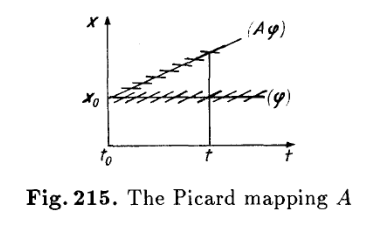
\includegraphics[width=\textwidth]{1-高维常微分方程-2025051316.png}
% \caption{}
\label{}
\end{figure}

To prove convergence of the successive approximations we shall construct a complete metric space in which the Picard mapping is a contraction.

The mapping $A:(M_1,\rho_1)\to (M_2,\rho_2)$ satisfies a \textbf{Lipschitz condition} with constant $L$ provided that
\[
\rho_2(Ax,Ay)\leq L\rho_1(x,y)\qquad \forall x,y\in M_1
\]
Let $\boldsymbol{f}:U\subset \mathbb{R}^{m}\to \mathbb{R}^{n}$ be a $C^{r}$ - mapping ($r\geq1$). Naturally, the derivative of $\boldsymbol{f}$ at $\boldsymbol{x}\in U\subset \mathbb{R}^{m}$
\[
\boldsymbol{f}_{*\boldsymbol{x}}:T_{x}\mathbb{R}^{m}\to T_{\boldsymbol{f}(\boldsymbol{x})}\mathbb{R}^{n}
\]
is a linear operator. If we choose a basis for each tangent space, $\boldsymbol{f}_{*\boldsymbol{x}}$ has a $m\times n$ matrix representation.

\begin{note}
$\boldsymbol{f}_{*\boldsymbol{x}}$ provides the best linear approximation of $\boldsymbol{f}(\boldsymbol{x})$ at the neighborhood of $\boldsymbol{x}$, i.e. $\boldsymbol{f}(\boldsymbol{x}+\boldsymbol{h})\approx \boldsymbol{f}(\boldsymbol{x})+\boldsymbol{f}_{*\boldsymbol{x}}(\boldsymbol{h})$.
\end{note}
\begin{figure}[H]
\centering
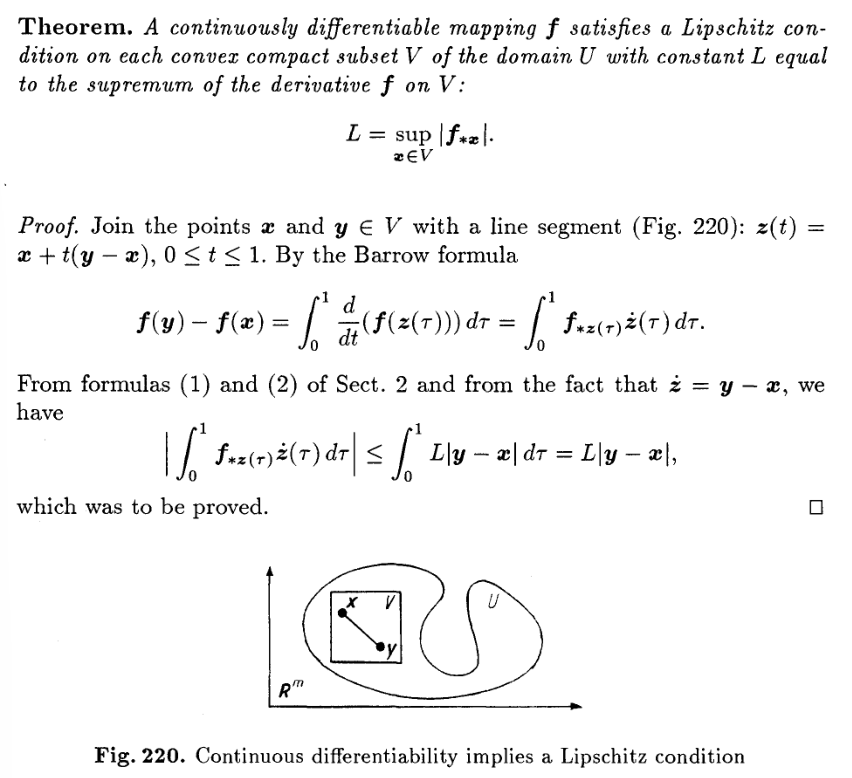
\includegraphics[width=\textwidth]{高维常微分方程-2025051317.png}
% \caption{}
\label{}
\end{figure}

\begin{remark}
By hypothesis $\boldsymbol{f}\in C^{1}$, $\boldsymbol{f}_{*\boldsymbol{x}}$ is continuous; then $\lvert \boldsymbol{f}_{*\boldsymbol{x}} \rvert$ attains a maximum value $L$ on any compact set $V$.
\end{remark}
See arnold for the proof of theorem of existence and uniqueness.

Next we consider the theorem on differentiablility. The motivation is as follows.

Associated with a differentiable mapping $f:U\to V$ is a linear operator on the tangent space
\[
f_{*}:TU\to TV
\]
At each point $x\in U$, $f_{*x}:T_{x}U\to T_{f(x)}V$.

In exactly the same way with a differential equation
\begin{equation}
\dot{\boldsymbol{x}}=\boldsymbol{v}(t,\boldsymbol{x})\qquad \boldsymbol{x}\in U\subset \mathbb{R}^{n}
\label{e0c026}
\end{equation}

there is associated a system of differential equations
\begin{equation}
\begin{cases}
\dot{\boldsymbol{x}}=\boldsymbol{v}(t,\boldsymbol{x}) & \boldsymbol{x}\in U\subset \mathbb{R}^{n} \\
\dot{\boldsymbol{y}}=\boldsymbol{v}_{*}(t,\boldsymbol{x})\boldsymbol{y} & \boldsymbol{y}\in T_{\boldsymbol{x}}U
\end{cases}
\label{90ff85}
\end{equation}

called the system of equations of variations for \cref{e0c026}, and linear w.r.t. the tangent vector $\boldsymbol{y}$.
\begin{figure}[H]
\centering
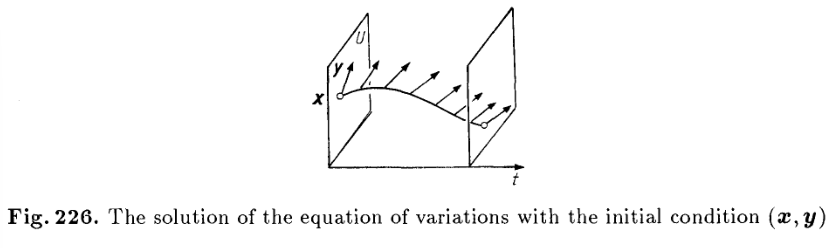
\includegraphics[width=\textwidth]{1-高维常微分方程-2025051317.png}
% \caption{}
\label{}
\end{figure}

We can correspond the unknown vector $\boldsymbol{y}$ to a unknown linear operator $z$.

\begin{figure}[H]
\centering
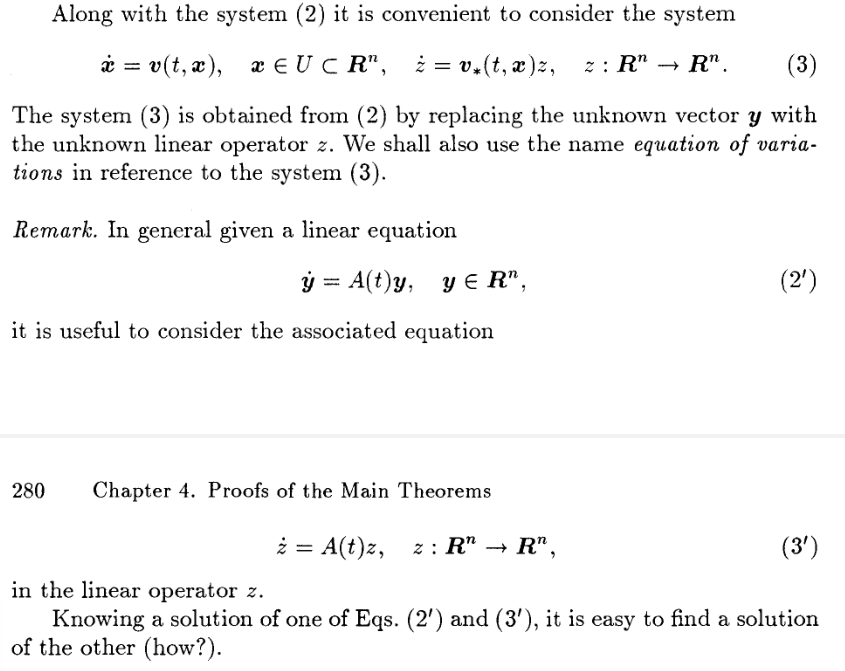
\includegraphics[width=\textwidth]{2-高维常微分方程-2025051317.png}
% \caption{}
\label{}
\end{figure}

\subsection{The differentiability theorem}

Suppose $\boldsymbol{v}$ of \cref{e0c026} is $C^{2}$ in some neighborhood of $(t_0,\boldsymbol{x}_{0})$. Then the solution $\boldsymbol{g}(t,\boldsymbol{x})$ of  \cref{e0c026} with initial condition $\boldsymbol{g}(t_0,\boldsymbol{x})=\boldsymbol{x}$ depends on the condition $\boldsymbol{x}$ in a continuously differentiable manner as $\boldsymbol{x}$ and $t$ vary in some neighborhood of $(t_0,\boldsymbol{x}_{0})$:
\[
\boldsymbol{v}\in C^{2}\Rightarrow \boldsymbol{g}\in C^{1}_{\boldsymbol{x}}
\]
\begin{figure}[H]
\centering
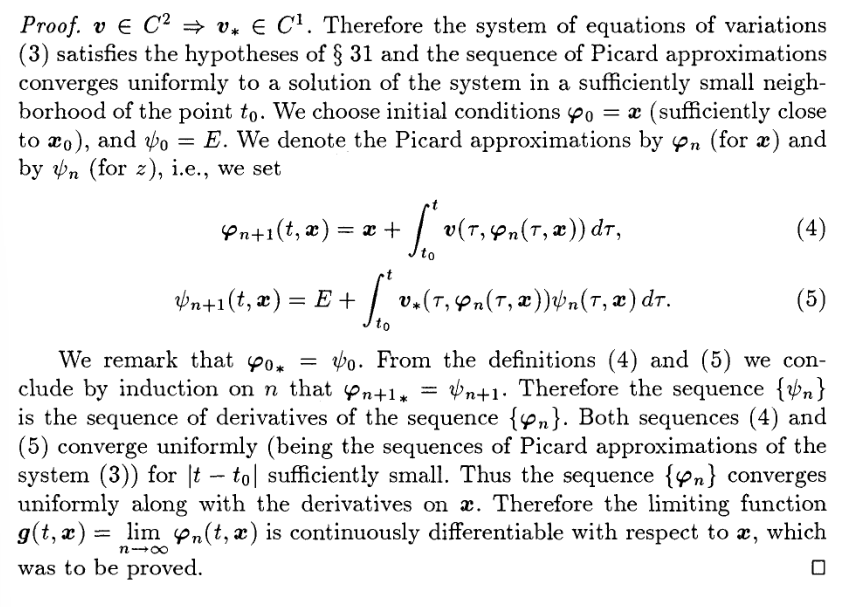
\includegraphics[width=\textwidth]{3-高维常微分方程-2025051317.png}
% \caption{}
\label{}
\end{figure}

\begin{figure}[H]
\centering
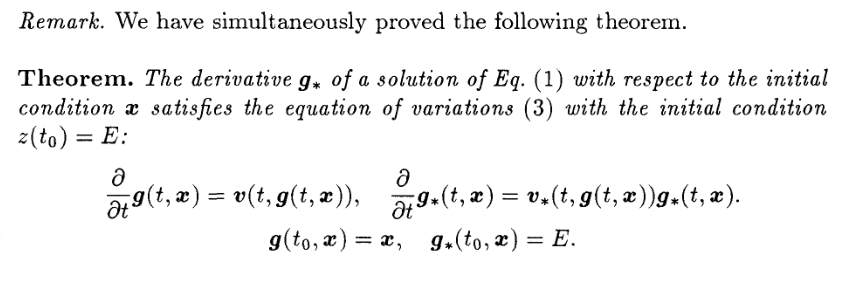
\includegraphics[width=\textwidth]{5-高维常微分方程-2025051317.png}
% \caption{}
\label{}
\end{figure}
This theorem explains the meaning of the equations of variations: they describe the action of the transformation over the time from $t_0$ to $t$ on the vectors tangent to the phase space (Fig. 227).
\begin{figure}[H]
\centering
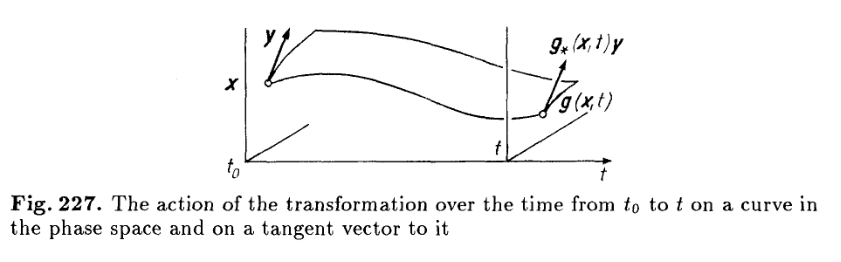
\includegraphics[width=\textwidth]{6-高维常微分方程-2025051317.png}
% \caption{}
\label{}
\end{figure}

More generally,
\[
\boldsymbol{v}\in C^{r}\Rightarrow \boldsymbol{g}\in C^{r-1}_{\boldsymbol{x}}
\]
We prove by induction
\[
\boldsymbol{v}\in C^{r}\Rightarrow \boldsymbol{v}_{*}\in C^{r-1}\overset{ \text{hypotheses} }{ \Rightarrow  }\boldsymbol{g}_{*}\in C^{r-2}_{\boldsymbol{x}}\Rightarrow \boldsymbol{g}\in C^{r-1}_{\boldsymbol{x}}
\]
In fact, we have
\[
\boldsymbol{v}\in C^{1}\Rightarrow \boldsymbol{g}\in C^{1}_{\boldsymbol{x}}
\]
\begin{figure}[H]
\centering
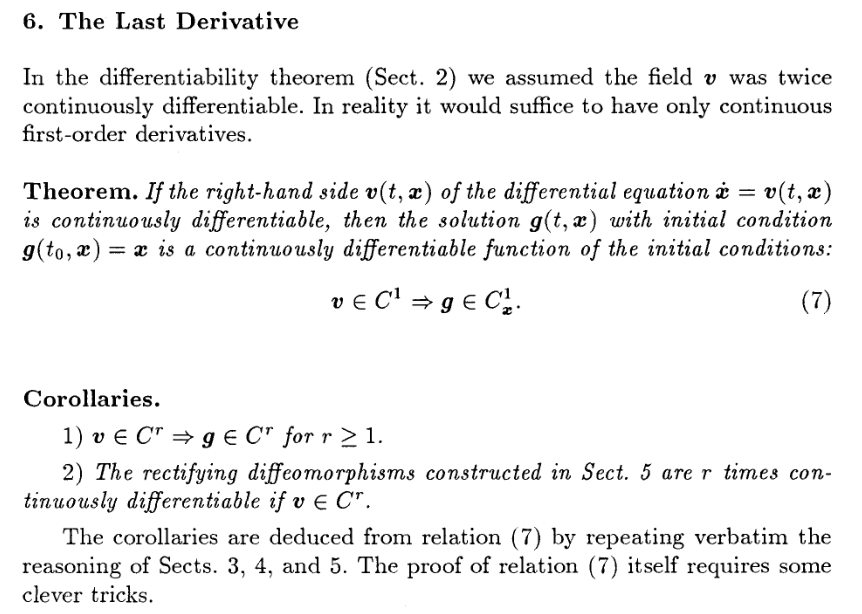
\includegraphics[width=\textwidth]{高维常微分方程-2025051318.png}
% \caption{}
\label{}
\end{figure}

\begin{lemma}
The solution of a linear equation
\[
\dot{\boldsymbol{y}}=A(t)\boldsymbol{y}
\]whose right-hand side depends continuously on $t$, exists; is unique; is determined uniquely by the initial conditions $\boldsymbol{\varphi}(t_0)=\boldsymbol{y}_{0}$; is a continuous function of $\boldsymbol{y}_{0}$ and $t$; is a \textbf{linear function} of $\boldsymbol{y}_{0}$ and a continuously differentiable function of $t$, thus $C^{1}$ in $\boldsymbol{y}_{0}$ and $t$.
\end{lemma}
\begin{lemma}
The solution of a linear equation
\[
\dot{\boldsymbol{y}}=A(t,\alpha)\boldsymbol{y}
\]where $A(t,\alpha)$ is continuous, is a continuous function of $\boldsymbol{y}_{0}$, $t$, and $\alpha$.\label{2cddf1}
\end{lemma}

We now apply \cref{2cddf1} to the equation of variations, \cref{90ff85} .

The system of equations of variations
\[
\dot{\boldsymbol{x}}=\boldsymbol{v}(t,\boldsymbol{x}),\qquad \dot{\boldsymbol{y}}=\boldsymbol{v}_{*}(t,\boldsymbol{x})\boldsymbol{y}
\]
has a solution uniquely determined by its initial data and depends continuously on them provided $\boldsymbol{v}\in C^{1}$.
